\documentclass[11pt, aspectratio=169]{beamer}

\usetheme{Madrid}
\usecolortheme{whale}

\usepackage{iftex}
\ifPDFTeX
\usepackage[T1]{fontenc}
\usepackage[utf8]{inputenc}
\usepackage[english]{babel}
\else
\usepackage{fontspec}
\usepackage[english, bidi=basic, provide=*]{babel}
\babelprovide[import, onchar=ids fonts]{english}
\babelfont{rm}{Noto Serif}
\babelfont{sf}{Noto Sans}
\babelfont{tt}{Noto Sans Mono}
\fi

\usepackage{booktabs}
\usepackage{amsmath}
\usepackage{graphicx}

\title[F-REGAL Final]{F-REGAL: Federated Graph Alignment}
\subtitle{Proof of Concept with PubMed, REGAL, and FedAvg Integration}
\author[Rushing \& Williams]{Adrian Rushing \and Joseph Williams}
\date{\today}

\begin{document}

\begin{frame}
    \titlepage
\end{frame}

\begin{frame}{Problem and Goal}
    \begin{itemize}
        \item In federated graph learning, clients cannot share raw graphs, so cross-silo node correspondence is hard.
        \item Existing FL methods can train models, but do not directly solve node-to-node alignment.
        \item We target a practical question: can we align nodes across private silos while preserving useful privacy constraints?
    \end{itemize}
    \vspace{0.25cm}
    \textbf{Goal:} Build a baseline pipeline that performs federated alignment and supports downstream GNN training.
\end{frame}

\begin{frame}{Implementation Difficulties}
    \begin{itemize}
        \item \textbf{No raw graph sharing:} privacy policies block sharing edges and local neighborhoods.
        \item \textbf{Heterogeneous silos:} clients have different graph slices and label distributions.
        \item \textbf{Alignment requirement:} downstream learning improves if equivalent nodes are matched across silos.
        \item \textbf{Tradeoff:} stronger privacy protection can distort alignment signal.
    \end{itemize}
\end{frame}

\begin{frame}{Method Summary: F-REGAL}
    \begin{itemize}
        \item \textbf{Local structural identity:} each client computes $k$-hop degree-based fingerprints.
        \item \textbf{Shared latent space:} clients map fingerprints to a common basis using xNetMF-style similarity projection.
        \item \textbf{Server alignment:} nearest-neighbor search (KD-tree) produces cross-client node matches.
        \item \textbf{Privacy mechanism:} optional Laplacian noise added to shared embeddings before alignment.
    \end{itemize}
    \vspace{0.2cm}
    Core projection form used in notebook:
    \[
    Y = C U \sqrt{\Sigma}
    \]
\end{frame}

\begin{frame}{Client and Server Roles}
    \begin{columns}[T]
        \begin{column}{0.48\textwidth}
            \textbf{Client-side (private)}
            \begin{itemize}
                \item Build local adjacency-derived descriptors.
                \item Combine structural and attribute features.
                \item Project to shared space using server basis.
                \item Optionally add Laplacian DP noise.
            \end{itemize}
        \end{column}
        \begin{column}{0.48\textwidth}
            \textbf{Server-side (coordinator)}
            \begin{itemize}
                \item Set global config and landmark basis.
                \item Broadcast projection metadata.
                \item Receive only transformed representations.
                \item Run KD-tree alignment and report matches.
            \end{itemize}
        \end{column}
    \end{columns}
\end{frame}

\begin{frame}{Implementation: Dataset, Client, Server}
    \begin{columns}[T]
        \begin{column}{0.33\textwidth}
            \textbf{Dataset}
            \begin{itemize}
                \item PubMed from \texttt{Planetoid}
                \item Undirected NetworkX graph
                \item Two client subgraphs sampled at 85\% node coverage each
            \end{itemize}
        \end{column}
        \begin{column}{0.33\textwidth}
            \textbf{Client}
            \begin{itemize}
                \item Extract structural identity ($K=2$, $\delta=0.5$)
                \item Fuse structure + attributes
                \item Build local similarity matrix $C$
                \item Optional DP noise ($b=0.05$)
            \end{itemize}
        \end{column}
        \begin{column}{0.33\textwidth}
            \textbf{Server}
            \begin{itemize}
                \item Build basis from 250 landmarks
                \item Compute global projection parameters $(U,\Sigma)$
                \item Align embeddings with top-1 nearest neighbor
            \end{itemize}
        \end{column}
    \end{columns}
\end{frame}

\begin{frame}{Configuration Used}
    \begin{itemize}
        \item Structural extraction depth and decay: $K=2$, $\delta=0.5$.
        \item Shared landmark basis size: 250 proxy nodes.
        \item Two privacy settings tested:
        \begin{itemize}
            \item Utility bound: DP scale $=0.0$.
            \item Privacy bound: DP scale $=0.05$.
        \end{itemize}
        \item Alignment metric: top-1 nearest-neighbor correctness on overlapping nodes.
    \end{itemize}
\end{frame}

\begin{frame}{Experiment Design}
    \begin{itemize}
        \item \textbf{Scenario A (Utility Bound):} no noise, clients share clean projected representations.
        \item \textbf{Scenario B (Privacy Bound):} Laplacian noise injected before sharing.
        \item Evaluate alignment only on true overlap nodes across client subgraphs.
        \item Then feed aligned representations into a two-layer GCN and run FedAvg rounds.
    \end{itemize}
    \vspace{0.2cm}
    FedAvg settings used in notebook:
    \begin{itemize}
        \item 30 rounds, 5 local epochs, Adam with weight decay.
    \end{itemize}
\end{frame}

\begin{frame}{Experiment Chart}
    \centering
    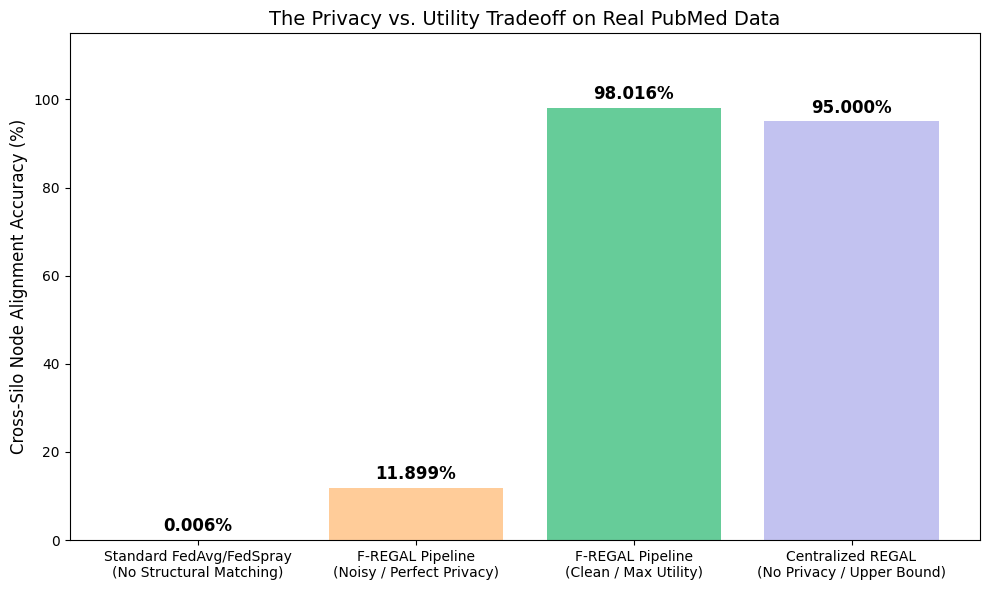
\includegraphics[width=0.92\textwidth,height=0.78\textheight,keepaspectratio]{chart.png}
\end{frame}

\begin{frame}{Results: Alignment Quality}
    \begin{table}
        \centering
        \begin{tabular}{@{}lc@{}}
            \toprule
            \textbf{Condition} & \textbf{Observed Outcome} \\
            \midrule
            Standard FL without explicit matching & Near-random alignment baseline \\
            F-REGAL (no noise) & \textbf{~98\% alignment accuracy} \\
            F-REGAL (+ Laplacian noise) & Noticeable drop from clean setting \\
            Centralized REGAL reference & High alignment (used as upper-bound context) \\
            \bottomrule
        \end{tabular}
    \end{table}
    \vspace{0.2cm}
    Result: F-REGAL solves the federation gap in clean settings, but privacy protection introduces a utility tax.
\end{frame}

\begin{frame}{Results: Downstream FedAvg Signal}
    \begin{itemize}
        \item Aligned representations were used as node features in a two-layer GCN.
        \item Federated averaging ran for 30 rounds with local client updates.
        \item Global model performance was tracked on client-local blind test partitions.
        \item This shows alignment is not only measurable, but useful for downstream learning workflows.
    \end{itemize}
\end{frame}

\begin{frame}{Interpretation: Why Privacy Is Not Free}
    \begin{itemize}
        \item Clean embeddings preserve fine structural signal, enabling near-centralized matching quality.
        \item DP noise improves resistance to reconstruction/triangulation attacks.
        \item The same noise perturbs nearest-neighbor geometry, reducing alignment precision.
    \end{itemize}
    \vspace{0.2cm}
    Practical objective is a tuned midpoint: enough blur for privacy, enough signal for alignment and learning.
\end{frame}

\begin{frame}{Shortcomings and Baseline Status}
    \begin{block}{Current limitations}
        \begin{itemize}
            \item This is a baseline proof of concept, not a fully production-hardened privacy system.
            \item Shared embeddings can still leak information under strong adversarial assumptions.
            \item Privacy is improved, but full formal end-to-end privacy guarantees are not yet ensured.
            \item Results are from one main dataset setup and should be stress-tested under broader non-IID settings.
        \end{itemize}
    \end{block}
\end{frame}

\begin{frame}{Threat Model and Privacy Gap}
    \begin{itemize}
        \item Assumed defense: embedding perturbation via Laplacian noise.
        \item Remaining risk: representation-level attacks may still infer sensitive structure.
        \item Missing today: formal privacy accounting tied to a concrete attacker capability model.
    \end{itemize}
    \vspace{0.25cm}
    \textbf{Key statement for this project:} this work is a proof of concept baseline and does \textbf{not} guarantee full privacy.
\end{frame}

\begin{frame}{Conclusion and Next Steps}
    \begin{itemize}
        \item F-REGAL demonstrates feasible federated node alignment with meaningful empirical gains.
        \item The project confirms a core tradeoff: stronger privacy noise lowers matching accuracy.
        \item Immediate next steps:
        \begin{itemize}
            \item calibrate DP across multiple scales and report full privacy-utility curves,
            \item extend evaluation across more datasets and client partitions,
            \item add stronger privacy accounting and attack-model testing.
        \end{itemize}
    \end{itemize}
\end{frame}

\begin{frame}
    \vspace{2cm}
    \begin{center}
        \Huge{\textbf{Questions?}} \\
        \vspace{1cm}
        \Large{Thank you.} \\
        \vspace{1.2cm}
        \normalsize{Adrian Rushing \& Joseph Williams}
    \end{center}
\end{frame}

\end{document}